\section{Phenix EMRinger protocol}
\label{app:emRingerProtocol}%a120
Protocol designed to assess the geometry of refined atomic structures regarding electron density maps in \scipion by using $EMRinger$ \citep{barad2015}. Integrated in cryo-EM validation tools of $Phenix$ software suite (\url{https://www.phenix-online.org/}) and created as an extension of the X-ray crystallography validation tool $Ringer$, $EMRinger$ tool computes the amount of rotameric angles of the structure side chains as a function of map value to assess the goodness of the fitting to the cryo-EM density map.

\begin{itemize}
 \item Requirements to run this protocol and visualize results:
    \begin{itemize}
        \item \scipion plugin: \ttt{scipion-em}
        \item \scipion plugin: \ttt{scipion-em-phenix}
        \item PHENIX software suite (tested for versions 1.13-2998, 1.16-3549, 1.17.1-3660 and 1.18.2-3874)
        \item \scipion plugin: \ttt{scipion-em-chimera}
    \end{itemize}
 \item \scipion menu:
  \ttt{Model building -> Validation} (\ffigure{fig:app_protocol_emringer_1} (A))
  
 \item Protocol form parameters (\ffigure{fig:app_protocol_emringer_1} (B)):
  
    \begin{figure}[H]
     \centering 
     \captionsetup{width=.9\linewidth} 
     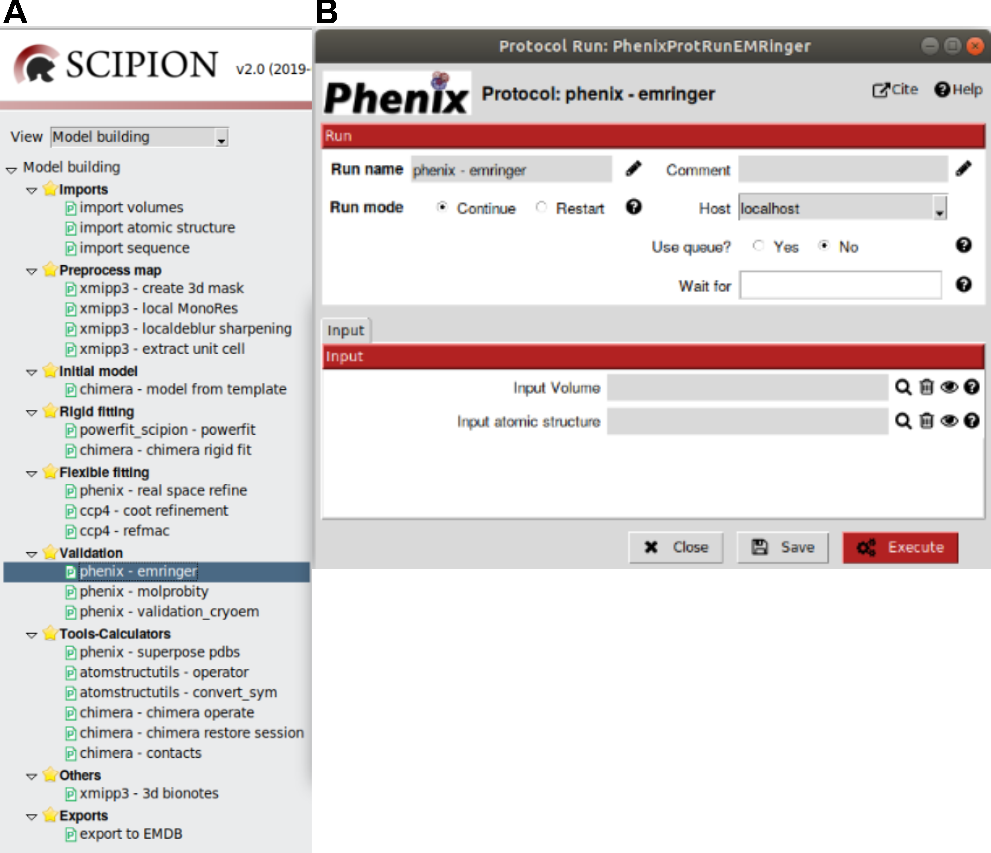
\includegraphics[width=0.90\textwidth]{Images_appendix/Fig139.pdf}
     \caption{Protocol \scommand{phenix - emringer}. A: Protocol location in \scipion menu. B: Protocol form.}
     \label{fig:app_protocol_emringer_1}
    \end{figure}

    \begin{itemize}
     \item \ttt{Input Volume}: Electron density map previously downloaded or generated in \scipion.
     \item \ttt{Input atomic structure}: Atomic structure previously downloaded or generated in \scipion and fitted to the input electron density map.
    \end{itemize}
    
 \item Protocol execution:

  Adding specific map/structure label is recommended in \ttt{Run name} section, at the form top. To add the label, open the protocol form, press the pencil symbol on the right side of \ttt{Run name} box, complete the label in the new opened window, press OK and, finally, close the protocol. This label will be shown in the output summary content (see below). If you want to run again this protocol, do not forget to set to \ttt{Restart} the \ttt{Run mode}.\\
  Press the \ttt{Execute} red button at the form bottom.
  
 \item Visualization of protocol results:
  
  After executing the protocol, press \ttt{Analyze Results} and the results window will be opened (\ffigure{fig:app_protocol_emringer_2}). 
  
  \begin{figure}[H]
     \centering 
     \captionsetup{width=.9\linewidth} 
     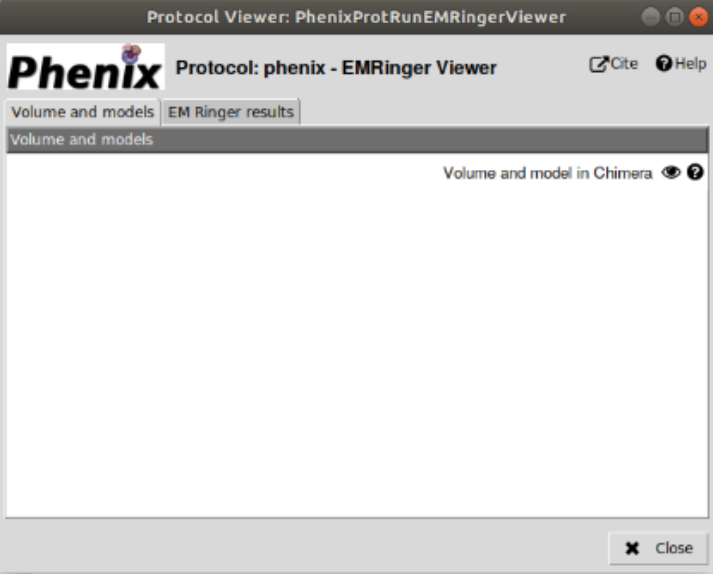
\includegraphics[width=0.50\textwidth]{Images_appendix/Fig140.pdf}
     \caption{Protocol \scommand{phenix - emringer}. Taps to visualize Volume and models and $EMRinger$ results.}
     \label{fig:app_protocol_emringer_2}
    \end{figure}
    
   Two taps are shown in the upper part of the results window:
    \begin{itemize}
     \item \ttt{Volume and models}: \chimera graphics window will be opened by default. Atomic structure and volume are referred to the origin of coordinates in \chimera. To show the relative position of atomic structure and electron density volume, the three coordinate axes are represented; X axis (red), Y axis (yellow), and Z axis (blue) (\ffigure{fig:app_protocol_volume_3}).

     \item \ttt{EMRinger Results} (\ffigure{fig:app_protocol_emringer_3}):
     
     \begin{figure}[H]
     \centering 
     \captionsetup{width=.9\linewidth} 
     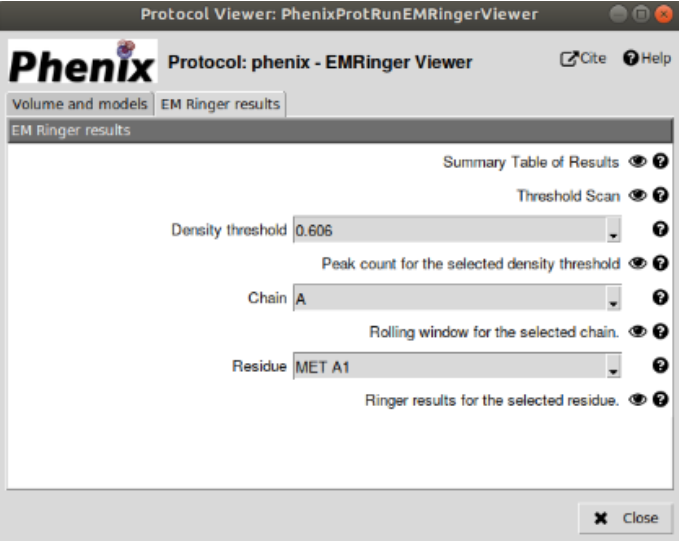
\includegraphics[width=0.50\textwidth]{Images_appendix/Fig141.pdf}
     \caption{Protocol \scommand{phenix - emringer}. Menu to visualize $EMRinger$ results.}
     \label{fig:app_protocol_emringer_3}
    \end{figure}
      \begin{itemize}
        \item \ttt{Summary Table of Results} (\ffigure{fig:app_protocol_emringer_4}):
        \begin{figure}[H]
         \centering 
         \captionsetup{width=.9\linewidth} 
         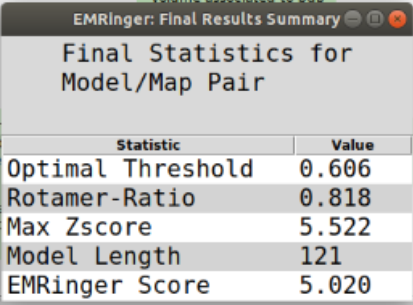
\includegraphics[width=0.40\textwidth]{Images_appendix/Fig142.pdf}
         \caption{Protocol \scommand{phenix - emringer}. Final $EMRinger$ results.}
        \label{fig:app_protocol_emringer_4}
     \end{figure}
         \begin{itemize}
          \item \ttt{Optimal Threshold}: \ttt{Electron Potential} cutoff value of the volume, in a range of 20, at which maximum values of \ttt{EMRinger Score} and \ttt{Percentage of Rotameric Residues} are reached. 
          \item \ttt{Rotamer-Ratio}: \ttt{Percentage of Rotameric Residues} at the \ttt{Optimal Threshold}.
          \item \ttt{Max Zscore}: Z-score indicating the significance of the distribution at the \ttt{Optimal Threshold}; in other words, probability of finding a certain number of rotameric residues at a specific side chain dihedral angle, among the total number of map peaks found above the \ttt{Optimal Threshold}, assuming a binomial distribution of rotameric residues B(\ttt{n, p)} ($n$: total number of map peaks found above the \ttt{Optimal Threshold}; $p$: 39/72; with map sampling every 5º, 39 angle binds are considered rotameric from a total of 360/5 = 72).
          \item \ttt{Model Length}: Total number of residues of the model considered in EMRinger computation, non-$\gamma$-branched, non-proline aminoacids with a non-H $\gamma$ atom.
          \item \ttt{EMRinger Score}: Highest Z-score, rescaled regarding model length, across the range of \ttt{Electron Potential} thresholds. Since the Z-score is rescaled to the \ttt{EMRinger Score} according model length, \ttt{EMRinger Score} allows suitable comparisons among different model-map pairs. \ttt{EMRinger Score} of 1.0 is usual for initial models refined regarding 3.2-3.5\AA\ resolution maps. For high-quality models with high resolution, \ttt{EMRinger Score} values higher than 2 are expected.
         \end{itemize}

        \item \ttt{Threshold Scan}: Plots of \ttt{EMRinger Score} (blue line) and \ttt{Percentage of Rotameric Residues} (red line) regarding the \ttt{Electron Potential} threshold. The maximum value of \ttt{EMRinger Score} stablishes the \ttt{Optimal Threshold}.
        \item \ttt{Density threshold}: Box to select one of the 20 volume density cutoff values at which the \ttt{Percentage of Rotameric Residues} has been computed. The \ttt{Optimal Threshold}, at which the \ttt{EMRinger Score} was obtained, is shown by default.
        \item \ttt{Peak count for the selected density threshold}: Histograms counting rotameric (blue) and non-rotameric (red) residues at the selected \ttt{Electron Potential Threshold}.
        \item \ttt{Chain}: Box to select one of the chains of the model. By default, the name of the first chain is shown.
        \item \ttt{Rolling window for the selected chain}: The analysis of EMRinger rolling window, performed on rolling sliding 21-residue windows along the primary sequence of monomers, allows to distinguish high quality regions of the model.
        \item \ttt{Residue}: Box to select one residue, with at least one \ttt{Chi} angle (non-H $\gamma$ atom-containing), located in the specific position indicated in the primary sequence of one of the monomer chains indicated.
        \item \ttt{Ringer results for the selected residue}: Individual plots for each \ttt{Chi} angle of the selected residue. Detailed numeric values are shown in the \ttt{extra/*.csv} file.
      \end{itemize}
    \end{itemize}
    
 \item Summary content:
 
  \ttt{SUMMARY} box:\\Statistics included in the above \ttt{Summary Table of Results} (an example can be observed in \ffigure{fig:emringer_protocol} (6).

\end{itemize}

